%==================Document Class and Packeges=====================
\documentclass[12pt,a4paper]{report}
\usepackage[T1]{fontenc}
\usepackage[utf8]{inputenc}
\usepackage[english]{babel}
\usepackage{amsmath,mathtools}
\usepackage{amsfonts}
\usepackage{amssymb}
\usepackage{graphicx}
\usepackage[left=1.5in,right=1in,top=2cm,bottom=2cm]{geometry}
	\graphicspath{{images/}}
\usepackage{times}
\usepackage{nomencl}
\usepackage[round]{natbib}
\usepackage{appendix}
\usepackage{setspace}
\usepackage{color}
\usepackage{fancybox}
\usepackage{lipsum}
\usepackage[bookmarks=true]{hyperref}
\usepackage{caption}
\usepackage{natbib}  % Bibliography
\usepackage{subcaption}
\usepackage{fancyhdr}
\usepackage{array}
\usepackage{multirow}
\pagestyle{fancy}
\usepackage{array}    % for Table array
\DeclareUnicodeCharacter{2212}{-}     %! Package inputenc Error: Unicode char − (U+2212)
\setlength{\parindent}{4em}           % Indentation
\setlength{\parskip}{1em}             % Spacing after paragraph
\renewcommand{\baselinestretch}{1.5}  % For Spacing
\usepackage{array}
\usepackage{multirow}

%==================Edited Commands and Pagelayouts=====

\fancyhead{}
\fancyhead[RO,LE]{Image Enhancement}
\fancyfoot{}
\fancyfoot[LE,RO]{\thepage}
\fancyfoot[LO,CE]{Chapter \thechapter}
\fancyfoot[CO,RE]{Priyanka B. Waghmode}

%\fancyhf{}
%\fancyhead[RO,LE]{Thesis Title}
%\fancyhead[LE,RO]{\thepage}
%\fancyhead[RE]{\it{\nouppercase{\leftmark}}}
%\fancyhead[LO]{\it{\nouppercase{\rightmark}}}
%\fancyfoot[CE,CO]{\small GF's Godavari College of Engg., Jalgaon}
%======================================================


\begin{document}

%=============Front Matters============================
%title
%dedication
%declaration
%Ack
%abstract
\begin{titlepage}

\newcommand{\HRule}{\rule{\linewidth}{0.5mm}} % Defines a new command for the horizontal lines, change thickness here

\center % Center everything on the page

%----------------------------------------------------------------------------------------
%	HEADING SECTIONS
%----------------------------------------------------------------------------------------

\textsc{\normalsize Image Enhancement Using Retinex Model}\\[1.5cm] % Name of your university/college
\normalsize Dissertation Submitted to the\\[0.5cm] % Major heading such as course name
\textsc{\normalsize NORTH MAHARASHTRA UNIVERSITY, Jalgaon}\\[0.5cm] % Minor heading such as course title
\normalsize For the Degree of\\[0.25cm]
\normalsize Master of Engineering\\[0.5cm]
\normalsize in\\[0.5cm]
\normalsize Computer Science and Engineering\\[0.5cm]
\normalsize By\\[0.5cm]
\textsc{\normalsize Priyanka B. Waghmode}\\[0.25cm]
\normalsize (ME(Computer)/2018-19/03)\\[0.5cm]
\normalsize Under the Guidance of\\
\textsc{\normalsize Prof. Nilesh Vani }\\
\normalsize Department of Computer Engineering
%----------------------------------------------------------------------------------------
%	TITLE SECTION
%----------------------------------------------------------------------------------------

%\HRule \\[0.4cm]
%{ \huge \bfseries Title}\\[0.4cm] % Title of your document
%\HRule \\[1.5cm]

%----------------------------------------------------------------------------------------
%	AUTHOR SECTION
%----------------------------------------------------------------------------------------

%\begin{minipage}{0.4\textwidth}
%\begin{flushleft} \large
%\emph{Author:}\\
%John \textsc{Smith} % Your name
%\end{flushleft}
%\end{minipage}
%~
%\begin{minipage}{0.4\textwidth}
%\begin{flushright} \large
%\emph{Supervisor:} \\
%Dr. James \textsc{Smith} % Supervisor's Name
%\end{flushright}
%\end{minipage}\\[2cm]


% If you don't want a supervisor, uncomment the two lines below and remove the section above
%\Large \emph{Author:}\\
%John \textsc{Smith}\\[3cm] % Your name

%----------------------------------------------------------------------------------------
%	DATE SECTION
%----------------------------------------------------------------------------------------

%{\large \today}\\[2cm] % Date, change the \today to a set date if you want to be precise

%----------------------------------------------------------------------------------------
%	LOGO SECTION
%----------------------------------------------------------------------------------------

 

\includegraphics[width=3cm]{logo.jpg}
%
\includegraphics{logo.jpg}\\[50mm] % Include a department/university logo - this will require the graphicx package

%----------------------------------------------------------------------------------------

\vfill % Fill the rest of the page with whitespace

\normalsize Godavari Foundation's\\[0.5cm]
\textsc{\normalsize Godavari College of Engineering, Jalgaon}\\[0.5cm]
\normalsize Maharashtra State, India\\[0.5cm]
\normalsize 2018-19\\[0.5cm]
\end{titlepage}
 

%========End Front Matters=============================

\begin{titlepage}

\newcommand{\HRule}{\rule{\linewidth}{0.5mm}} % Defines a new command for the horizontal lines, change thickness here

\center % Center everything on the page

%----------------------------------------------------------------------------------------
%	HEADING SECTIONS
%----------------------------------------------------------------------------------------

\textsc{\normalsize Image Enhancement Using Retinex Model}\\[1.5cm] % Name of your university/college
\normalsize Submitted By\\[0.5cm] % Major heading such as course name
\textsc{\normalsize PRIYANKA B. WAGHMODE}\\[0.5cm] % Minor heading such as course title
\normalsize In the partial fulfilment for the award of \\[1cm]
\normalsize Master of Engineering\\[0.1cm]
\normalsize (Computer Science and Engineering)\\[1cm]
\normalsize Guided By\\[0.5cm]
\textsc{\normalsize Prof. Nilesh Vani}\\[0.25cm]
\normalsize Department of Computer Engineering\\[0.5cm]

%----------------------------------------------------------------------------------------
%	TITLE SECTION
%----------------------------------------------------------------------------------------

%\HRule \\[0.4cm]
%{ \huge \bfseries Title}\\[0.4cm] % Title of your document
%\HRule \\[1.5cm]

%----------------------------------------------------------------------------------------
%	AUTHOR SECTION
%----------------------------------------------------------------------------------------

%\begin{minipage}{0.4\textwidth}
%\begin{flushleft} \large
%\emph{Author:}\\
%John \textsc{Smith} % Your name
%\end{flushleft}
%\end{minipage}
%~
%\begin{minipage}{0.4\textwidth}
%\begin{flushright} \large
%\emph{Supervisor:} \\
%Dr. James \textsc{Smith} % Supervisor's Name
%\end{flushright}
%\end{minipage}\\[2cm]


% If you don't want a supervisor, uncomment the two lines below and remove the section above
%\Large \emph{Author:}\\
%John \textsc{Smith}\\[3cm] % Your name

%----------------------------------------------------------------------------------------
%	DATE SECTION
%----------------------------------------------------------------------------------------

%{\large \today}\\[2cm] % Date, change the \today to a set date if you want to be precise

%----------------------------------------------------------------------------------------
%	LOGO SECTION
%----------------------------------------------------------------------------------------

 
%
\includegraphics[width=0.5cm]{logo.jpeg}
%
\includegraphics{logo.jpg}\\[50mm] % Include a department/university logo - this will require the graphicx package

%----------------------------------------------------------------------------------------

\vfill % Fill the rest of the page with whitespace

\normalsize Godavari Foundation's\\[0.5cm]
\textsc{\normalsize Godavari College of Engineering, Jalgaon}\\[0.5cm]
\normalsize Maharashtra State, India\\[0.5cm]
\normalsize 2018-19\\[0.5cm]
\end{titlepage}
 
\newpage
\thispagestyle{empty}

\begin{center}
\normalsize Godavari Foundation's\\
\huge{Godavari College of Engineering, Jalgaon}\\[0.5cm]
\normalsize
\textsc{Department of computer science and engineering}\\[2.0cm]

\emph{\LARGE Certificate}\\[2.5cm]
\end{center}
\normalsize This is to certify that this is a bonafide record of the project presented by the students whose names are given below during <Monsoon/Winter and Year here> in partial fulfilment of the requirements of the degree of Bachelor of Technology in Computer Science and Engineering.\\[1.0cm]

\begin{table}[h]
	\centering
	\begin{tabular}{m{10cm} m{4cm}}%{lr}

		Prof. Nilesh Vani & Prof. Rahul Gaikwad \\ 
		Guide & ME Coordinator \\  \\  \\  \\  \\
		Prof. Pramod Giri & Prof. Dr.  \\
		Head of Department & Principal
	\end{tabular}
\end{table}

\vfill


% Bottom of the page
%\begin{flushright}
%<Guide name here>\\
%(Project Guide)\\[1.5cm]
%<Coordinator name here>\\
%(Course Coordinator)\\
%\end{flushright}

\begin{flushleft}
Date:
\end{flushleft}
\newpage
\thispagestyle{empty}

\begin{center}
\emph{\LARGE Declaration}\\[2.5cm]
\end{center}

\normalsize I hereby declare that I have formed, completed and written the dissertation entitled " Enhancement of Low Light Images Via Illumination Map Estimation Using Variational Optimization based Retinex Models". It has not previously submitted for the basis of the award of any degree or diploma or other similar title of this for any other examining body or University.
\begin{flushleft}
Place:\\
Date:
\end{flushleft}




% Bottom of the page
\begin{flushright}
Priyanka B. Waghmode\\
Student ME(Computer)\\[1.5cm]
%<Coordinator name here>\\
%(Course Coordinator)\\
\end{flushright}


\newpage
\thispagestyle{empty}

\begin{center}
\emph{\LARGE Dissertation Approval Sheet}\\[2.5cm]
\end{center}

\normalsize This is to certify that this is a bonafide record of the project presented by the students whose names are given below during <Monsoon/Winter and Year here> in partial fulfilment of the requirements of the degree of Bachelor of Technology in Computer Science and Engineering.\\[1.0cm]

\begin{flushleft}
Place:\\
Date:
\end{flushleft}







% Bottom of the page
\begin{flushleft}
Guide: Prof. Nilesh Vani\\[2cm]
External Examiner\\[1.5cm]
Place:\\
Department of Computer Engineering\\
Godavari College of Engineering, Jalgaon(M.S.) 
\end{flushleft}


\newpage
\thispagestyle{empty}

\begin{center}
\emph{\LARGE Acknowledgement}\\[2.5cm]
\end{center}

\normalsize I would like to acknowledge my indebtedness and render my warmest thanks
to my guide \textbf{prof. Nilesh Vani}, who made this work possible. His friendly guidance and expert advice have been invaluable throughout all stages of the work. I would also wish to express my gratitude to my Head of Department \textbf{Prof. Pramod Gosavi} for extended discussions and valuable suggestions which have contributed greatly to the improvement of the thesis. The thesis has also benefited from comments and suggestions made by \textbf{Prof. Rahul Gaikwad} who have read through the manuscript. I take this opportunity to thank them.My special thanks are extended to my \textbf{Principal Prof. (Dr) V. G. Arajpure}, for the drawing on the cover.

Special thanks are due to my husband, \textbf{Mr. Harish Gadade}, for his continuous support and understanding, but also for more concrete thinks like commenting on earlier versions of the thesis, helping with the figures and the final preparation of the manuscript. I want to thank my friend \textbf{Tasneem} and my sisters \textbf{Rituja} and \textbf{Snehal}, for constant encouragement. I would like to thank the Computer Department of my college for providing excellent working conditions. Also I thank all those who have supported me directly or indirectly\\[1.0cm]





% Bottom of the page
\begin{flushright}
Priyanka B. Waghmode\\
Student Computer science and Engg.\\
Godavari College of Engineering, Jalgaon(M.S.) 
\end{flushright}


\newpage
\thispagestyle{empty}

\begin{center}
\emph{\LARGE Abstracts}\\[2.5cm]
\end{center}

\normalsize Image Enhancement is one of the important requirements in Digital Image
Processing which is very important in making an image useful for various applications which can be seen in the areas of Video Surveillance, Digital photography, Medicine, Geographic Information System, Industrial Inspection , Law Enforcement and many more Digital Image Applications. Image Enhancement is used to improve the quality of poor images. The focus of this dissertation is an attempt to improve the quality of digital images using various Retinex Model like Single Scale Retinex Model, Multi-Scale Retinex Model,Multi-Scale Retinex Model with color Restoration. Also this dissertation focused on Power Law Transformation, Histogram Equalization and Adaptive Histogram Equalization. In this dissertation i have applied various Retinex Model, Power Law Transformation,Histogram Equalization and Adaptive Histogram Equalization on color images with different color space.\\\\
\textbf{Keyword:} Retinex Algorithm, SSR,MSR,MSRCR,Hostogram,Image Enhancement. \\[1.0cm]









%======================================================

\tableofcontents


\listoffigures


\listoftables

%=====================Main Matters====================
\chapter{Introduction}
Retinex  Theory was formulated by Edwin H. Land In 1964. His theory and an extension, the “reset Retinex” were further formalized by Land and Mc Cann [1]. It was the first attempt to simulate and explain the human visual system how it perceives colours, based on experiments using Mondrian patterns.
\section{Introduction}
Besides digital photography, retinex algorithms are used to make the information in astronomical photos visible and detect, in medicine, poorly visible structures in X-rays or scanners. In brief it helps to achieve many features such as sharpening, colour constancy processing and dynamic range compression [5]. The Retinex Image Enhancement Algorithm is an automatic image enhancement method that enhances a digital image in terms of dynamic range compression, colour independence from the spectral distribution of the scene illuminate, and colour/ lightness rendition. The digital image enhanced by the Retinex Image Enhancement Algorithm is much closer to the scene perceived by the human visual system, under all kinds and levels of lighting variations, than the digital image enhanced by any other method [6]. Image enhancement technology has permeated in many areas of science, engineering and civilian, such as biomedicine images, astrophotography, satellite pictures, computer vision, surveillance systems, civilian cameras, etc.[7]

\section{Problem Definition}
Our system will enhance the input image by applying retinex algorithms: Multi-Scale Retinex with color Restoration (MSRCR), Multi-scale Retinex with Chromaticity Preservation (MSRCP) and Automated Multi-Scale Retinex with Color Restoration (AMSRCR). Thus, the Problem definition can be proposed as follows: To implement the Algorithms: MSRCR, MSRCP and AMSRCR. Also, these algorithms require implementation of Single-Scale Retinex (SSR) algorithm and the SimplestColorBalance algorithm [35].
\section{Objective}
	\begin{itemize}
		\item To implement Single-Scale Retinex and Color Restoration Algorithms.
		\item To implement Multi-Scale Retinex with Color Restoration using above 
		algorithms (MSRCR).
		\item To implement Multi-Scale retinex with Chromaticity preservation- MSRCP.(a 
		modified version of above algorithm).
		\item To implement Automated Multi-Scale Retinex with Color Restoration algorithm.	
		(An automated (image independent) approach to MSRCR)- AMSRCR.
	\end{itemize}
	
\section{Scope}
The Retinex Image Enhancement Algorithm is an automatic image enhancement method that enhances a digital image in terms of dynamic range compression, colour independence from the spectral distribution of the scene illuminate, and colour/ lightness rendition. So, the scope of this project is to implement the Retinex based image Enhancement Algorithms, which involves the implementation of following three models of retinex algorithms:
	\begin{itemize}
		\item Multi-Scale Retinex algorithm with color Restoration (MSRCR)
		\item Multi-Scale Retinex algorithm with Chromaticity Preservation (MSRCP)
		\item Automated Multi-Scale Retinex algorithm with Color Restoration (AMSRCR)

	\end{itemize}
\section{Existing System}
The existing image enhancement techniques like auto gain/offset, gamma correction, histogram equalization and homomorphic filtering heavily depend on input images. For auto gain/offset, it could achieve dynamic range compression but at the loss of details due to saturation and clipping. For gamma correction, it is good to improve pictures either too dark or too bright but it is a global function applied to the picture, thus there is no enhancement involved. For histogram equalization and homomorphic filtering, they all failed for bi-modal pictures, which include both dark and bright areas. But for retinex, it could achieve satisfactory results for both pictures, thus its benefits are obviously to see.[8]
\section{Outline}
This project report is organized into six chapters: Chapter 1 introduces the project; chapter 2 describes related work and reviews previous works; Chapter 3 presents the technology that will be used. Chapter 4 presents the system analysis and design in detail, chapter 5 presents the results and Chapter 6 is the Conclusion.
\chapter{Related Work}
The Retinex Image Enhancement Algorithm is an automatic image enhancement method that enhances a digital image in terms of dynamic range compression, colour independence from the spectral distribution of the scene illuminate, and colour/ lightness rendition. There are several retinex based image Enhancement techniques. Some of them are described in this chapter.
\section{Image Processing}
Image processing is a method to perform some operations on an image, in order to get an enhanced image or to extract some useful information from it. It is a type of signal processing in which input is an image and output may be image or characteristics/features associated with that image. Nowadays, image processing is among rapidly growing technologies. It forms core research area within engineering and computer science disciplines too. Image processing basically includes the following three steps:
	\begin{itemize}
		\item Importing the image via image acquisition tools;
		\item Analysing and manipulating the image;
		\item Output in which result can be altered image or report that is based on image  		analysis.
	\end{itemize}
	
There are two types of methods used for image processing namely, analogue and digital image processing. Analogue image processing can be used for the hard copies like printouts and photographs. Image analysts use various fundamentals of interpretation while using these visual techniques. Digital image processing techniques help in manipulation of the digital images by using computers. The three general phases that all types of data have to undergo while using digital technique are pre-processing, enhancement, and display, information extraction[9]. In this project, we are working on the enhancement phase. Thus the following section focuses on the study of image enhancement.


\section{Image Enhancement Techniques}
Image enhancement techniques can be divided into two main categories:
\begin{itemize}
	\item Spatial Domain Method
	\item Frequency Domain Method
\end{itemize}
Spatial domain method directly deals with the pixel values of an image. Whereas Frequency domain method operates on Fourier transform of an image for enhancement of an image.


\subsection{Spatial Domain Technique}
The Spatial domain method is directly operated on pixels of an image. The pixel values are modified based on the problem domain. The objective of this method is to improve the perceptibility of information contained in an image and also enhancing the structural features can improve perceived image quality [10]. Spatial domain methods directly manipulate the image data array, either by point processing or area processing. Basically it deals with spatial frequency, i.e. difference between the highest and the lowest values of a contiguous set of pixels [11]. The technique regarding image enhancement using spatial domain methods can be divide into two categories -
	\begin{itemize}
		\item Global Image Enhancement
		\item Local Image Enhancement
	
	\end{itemize}
Global methods are mainly histogram modification that aims to exploit the full dynamic range of a rendering device by modifying the histogram of an image. The attractiveness is their simplicity and minor computational effort. However it is often necessary to enhance detail over a smaller area. So, the local image enhancement method plays a major role in those applications [11].\par 
Image processing is defined as the process of analysing and manipulating images using a computer. Using computer algorithms to perform image processing on digital images is referred as Digital image processing. Image Enhancement is simple and most appealing areas among all the digital image processing techniques. Image enhancement is to improve the image quality so that the resultant image is better than the original image for a specific application. Hence Image Enhancement is a “subjective process” which means that the human perception decides the best method from the obtained results. As we know that frequency domain methods first transform the images into transform domain or frequency domain and then operate on the transformed images. After the process, the images are transformed back to spatial domain by applying inverse transforms.[12]
There are many spatial domain techniques that are divided according to global or local image enhancement. Histogram Equalization is global image enhancement which is one of the simplest and widely used techniques. Histogram equalization is the technique by which the dynamic range of the histogram of an image is increased. It assigns the intensity values of pixels in the input image such that the output image contains a uniform distribution of intensities. It improves contrast and the goal of histogram equalization is to obtain a uniform histogram [14]. In HE, the cumulative density function (cdf) of the histogram is used as the intensity transfer function; this method enhances the contrast by distributing the cdf across the entire dynamic range. However, this even distribution creates artefacts’ in the smooth regions of the image. Moreover, it does not consider the boundaries, which degrades the sharpness of the resulting image [15].
When the original histogram does not occupy the entire dynamic range of the image, HE produces washout effect which is the disadvantage of HE. Thus there are several techniques which based on HE has been proposed to overcome the disadvantages of original technique. One of the techniques is Adaptive Histogram Equalization. Adaptive histogram Equalization is local image enhancement. This is an extension to traditional Histogram Equalization technique. It enhances the contrast of images by transforming the values in the intensity image Unlike HE it operates on small data regions (tiles), rather than the entire image. Each tile's contrast is enhanced, so that the histogram of the output region approximately matches the specified histogram. The neighbouring tiles are then combined using bilinear interpolation in order to eliminate artificially induced boundaries [14]. In AHE, histogram of image is divided into many modified to match across boundaries. It produces good result in dark images. The contrast, especially in homogeneous areas, can be limited in order to avoid amplifying the noise which might be present in the image. There are some other technique which based on spatial domain methods such as Bi-histogram equalization and Laplacian. BHE splits the histogram into two parts based on where the mean lies. Each part is then enhanced independently using HE. BHE maintains the intensity mean of the original image, which suppresses the over enhancement problem. Unnatural images are, however, still produced [13]. Laplacian is used to enhance the edges of an image thus it is edge enhancing algorithm. It perform local enhancement of the brightness levels of image pixels. Therefore the resultant image has increase in local contrast at boundaries rectangular domains, and then each domain is passed through the histogram equalization. Once this is completed the brightness levels are enhanced.  Table 2.1 shows the summary of spatial techniques[28].

\begin{table}[h!]
	\begin{center}
	\caption{Your first table.}
    \label{tab:table1}
	\begin{tabular}{ | m{4cm} | m{8cm}| }
	\hline
		Histogram Equalization & Adjusting the global contrast of an image. It is most effective method for gray scale images \\
	\hline
		Adaptive histogram Equalization & It is extension of HE and used within an image for local enhancement. It contains dark region and low contrast \\ 
	\hline
		Bi- histogram equalization & It maintains the intensity mean of the original image, which suppresses the over enhancement problem \\ 
	\hline
		Laplacian & It is mostly used for edge enhancement \\ 
	\hline
	\end{tabular}
	\end{center}

\end{table}

\subsection{Frequency Domain Technique}
Frequency domain method operates on the Fourier transform of an image. Image enhancement in the frequency domain is straightforward. We simply compute the Fourier transform of the image to be enhanced, multiply the result by a filter and take the inverse transform to produce the enhanced image. In frequency domain methods, the image is first transferred in to frequency domain. It means that, the Fourier Transform of the image is computed first. All the enhancement operations are performed on the Fourier transform of the image and then the Inverse Fourier transform is performed to get the resultant image. These enhancement operations are performed in order to modify the image brightness, contrast or the distribution of the grey levels. As a consequence the pixel value of the output image will be modified according to the transformation function applied on the input values [15]. The convolution theorem is the foundation of frequency domain techniques. Consider the following spatial domain operation:

\begin{equation}
	g(x,y)=h(x,y)*f(x,y)
\end{equation}

The following frequency domain relationship given by the convolution theorem 

\begin{equation}
	G (u, v) = H (u, v) F (U, v)
\end{equation}


Where g, f and h having Fourier transform G, H and F respectively. H is known as the transfer function of the process. Many image enhancement problems can be viewed in the form of the above equation. The main aim is to select a transfer function that changes the image in such a way that certain features of an image are enhanced. Examples: edge detection, noise removal.

There are mainly three types of filters
\begin{itemize}
	\item Low pass filter
	\item High pass filter
	\item Band pass filter

\end{itemize}

In Low-pass filtering, sharp transitions and edges in the gray levels of an image contribute significantly to the high frequency content of its Fourier Transform. By attenuating a specified range of high-frequency components in the frequency domain, blurring is achieved. Through Low-pass filtering this task is performed.

By High-pass filtering, Image sharpening can be achieved in the frequency domain. Low-frequency components will attenuated by high pass filter the without disturbing high frequency information.

Band-pass filtering is a method in which the reflectance and illumination components can be filtered independently. The illumination component of an image is generally classified by slow spatial variation on the other hand the reflectance component of an image tends to vary abruptly. These characteristics lead to associating the low frequencies of the Fourier transform of the natural log of an image with illumination and high frequencies with reflectance thus it is filtered individually.

\subsection{Comparison between Spatial Domain Technique And Frequency Domain Technique}
\begin{itemize}
	\item Spatial domain is manipulation of pixels of an image. It is the technique for changing the representation of an image and used in many field such as sharpening and smoothing images. Whereas Frequency domain is the manipulation of Fourier transforms to enhance an image and perform purely with convolution theorem and it is used in changing the position of an image. 
	\item The advantage of spatial domain technique is that it is simple to understand and the complexity of these techniques is very low which helps in real time implementation. Whereas Frequency domain technique having advantages which include low computation complexity, easy to view, manipulation of image’s frequency composition and the special transformed domain property is easily applicable.
	
\end{itemize}

The disadvantages of spatial domain technique is that it does not provides adequate robustness and perceivably. Whereas the disadvantage of Frequency Domain is that it cannot enhance properly every part of an image simultaneously and the automation of image enhancement is also very difficult. Table 2.2 shows the areas where Spatial Domain technique and Frequency domain technique are applied [16].

\begin{table}[h!]
	\begin{center}
	\caption{Your first table.}
    \label{tab:table1}
	\begin{tabular}{| m{5cm} | m{8cm}| }
	\hline
		\textbf{Techniques} & \textbf{Feature}\\
	\hline
		Spatial Domain technique & It is used to alter The gray level value Of individual pixels and hence the overall contrast of the entire image. It is not possible to selectively enhance edges or other required information effectively. \\
	\hline
		Frequency domain technique & It is used to Easily enhance edges And other subtle information because they are high frequency content and frequency domain operates on frequency content of an image. In this technique, all parts of  an  image  are  not enhanced in uniform manner \\ 
	
	\hline
	\end{tabular}
	\end{center}

\end{table}


\section{BASICS OF RETINEX THEORY}
Retinex is the theory of human color vision proposed by Edwin Land to account for color sensations in real scenes. Color constancy experiments showed that color does not correlate with receptor responses. In real scenes, the content of the entire image controls appearances. A triplet of L, M, S cone responses can appear any color. Land coined the word “Retinex” (the contraction of retina and cortex) to identify the spatial image processing responsible for color constancy. Further, he showed that color sensations are predicted by three lightnesses observed in long-, middle-, and short-wave illumination. Retinex is also used as the name of computer algorithms that mimic vision’s spatial interactions to calculate the lightnesses observed in complex scenes.

\subsection{Overview}
Edwin H. Land, the inventor of hundreds of film patents, was struck by experiments showing that color sensations in real complex images depend on scene content. Film responds to the light falling on each tiny local region. Land realized that vision’s mechanisms were very different from film. His early experiments studied the colors observed in red and white projections [1]. He realized color appearance required both the cone responses to a local region and the neural spatial processing of the rest of the scene. He proposed the Retinex Theory.

Land coined the word Retinex to describe three independent spatial channels. In 1964 he wrote: “We would propose that all of the receptors with maximum sensitivity to the long-waves in the spectrum, for example, operate as a unit to form a complete record of long-wave stimuli from objects being observed. (For convenience of reference, let us call this suggested retinal-cerebral system a “retinex.”)” [2, 3, 4, 5]. It is the word that describes the mechanism that performs the comparison of scene information to create the array of sensations of lightness in three channels


\subsection{Cone Quanta Catch}
Visible light falls on objects that reflect some of it to the eye. Color vision depends on the spectrum of the illumination falling on an object and the spectrum of its reflectance. The product of these spectra describes the light coming to the eye. There are three types of cones in normal observers that are called L for long-wave-, M for middle-wave-, and S for short-wave-sensitive cones. The receptors’ spectral sensitivities multiplied by the light falling on the retina determines the L, M, S cone responses, namely, the “quanta catch” of the cones. The cones convert the quanta catch to nerve signals that pass through many spatial comparisons in the visual system. The cone quanta catch is the important transition from the physics of light to the physiology of vision. However, it is just the first step in the process.
Figure 2.1 illustrates a laboratory experiment that generates equal L, M, S quanta catches from different reflectance papers.
Light passes through filters that determine the spectrum of each illumination falling on circular pieces of paper. The light coming to the eye from the papers is modified again by the reflectance spectra of the papers. Further, in this experiment there is no light coming from the black surrounds.
On the left, there is a tungsten light source at the top. There is a filter that absorbs more middle-wave than long- and short-wave visible light (magenta arrows). The green circular paper reflects more middle-wave than long- and short-wave light. The light coming to the eye is the product of these spectra. The integrals of that light using the three cone spectral sensitivities determine the L, M, S quanta catch values.


%\begin{figure}[h!]
 % 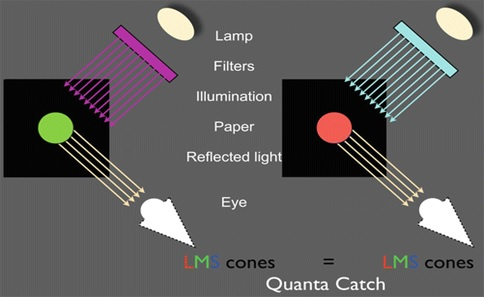
\includegraphics[width=1.7]{equalQuanta.jpg}
  %\caption{equalQuanta}
  	%\label{fig:equalQuanta}
%\end{figure}

%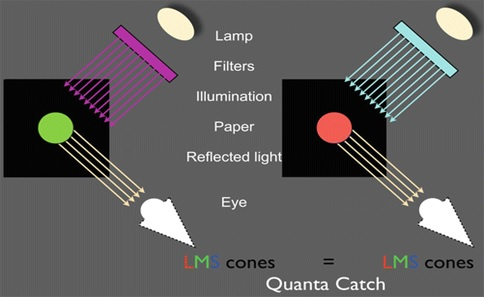
\includegraphics{{C:\Harish\Latex\Sample\equalQuanta.jpg}}

On the right, there is the same tungsten light source at the top. There is a different filter that absorbs more long-wave than middle- and short-wave light (cyan arrows). The right-red paper reflects more long-wave than middle- and short-wave light. In this experiment, the spectra of the two illuminants and the two reflectances were adjusted to generate the same triplet of LMS cone quanta catches. Under these conditions, the left-green and right-red papers are identical retinal stimuli. They appear equal to each other, but that color is neither red nor green.[17]

\subsection{Mondrian Experiments}
Land’s color Mondrian experiment is similar, with the exception that he used a complex array of papers to simulate real-world scenes. The important difference is that in complex scenes, a particular quanta catch can appear in any color: red, green, blue, yellow, white, or black.
Figure 2.2. shows the double color Mondrian experiment [6]. It used two identical Mondrians made of color papers, and three different, non-overlapping spectral illuminants (long-, middle-, and short-wave visible light). In this experiment observers reported the colors of papers in the Mondrians. In this illustration, we will look at the circular red and green papers. Land adjusted the illuminant mixtures of light from the two sets of three projectors. The same amounts of L, M, S light came from the green circle on the left as from the red circle on the right. First, he turned on just the long-wave lights. He adjusted the amounts of illumination on the left-green and right-red circles so the meter readings were equal. Then, he did the same for middle- and short-wave light. The left-green and right-red circles had equal quanta catches by the L, M, S cones.


%\begin{figure}[h!]
 % \includegraphics[width=1.7]{landsExperiments.jpg}
  %\caption{landsExperiments}
  	%\label{fig:equalQuanta}
%\end{figure}

Two identical sets of matte colored papers, with separate L, M, S illuminating projectors with voltage transformers for control of the amount of light. Telephotometer readings were projected above the Mondrians. The experimenter separately measured the L, M, S radiances from a green circle in the left Mondrian. Then, he adjusted the L, M, S radiances from a red circle on the right Mondrian to be the same. Observers reported different red and green colors produced by identical light stimuli.

In this complex scene, observers reported that equal quanta catches appeared green on the left and red on the right. Observers reported color constancy, namely, that the red paper looked red and the green paper looked green despite the identical cone quanta catch.

Land repeated this experiment with all the Mondrian papers. A constant L, M, S quanta catch could generate any color sensation. The presence of the complex scene introduced more information to the visual system. The red and green papers appeared equal in Fig. 2.1. The red paper looked red and the green paper looked green in Fig. 2.2. The scene’s spatial content stimulated vision’s spatial image processing mechanisms to generate color constancy. The post-receptor visual processing plays a dominant role in color appearance in real scenes. Land’s word “Retinex” gave this spatial process a name. As well, he proposed a theoretical mechanism.[17]

\subsection{Retinex Mechanism}
Figure 2.3. illustrates the pair of Mondrians in only long-wave light with more light on the left than on the right. Their appearances are nearly constant. This is a common observation: humans are insensitive to large changes in uniform illumination.

%\begin{figure}[h!]
 % \includegraphics[width=1.7]{landsExperiments.jpg}
  %\caption{landsExperiments}
  	%\label{fig:equalQuanta}
%\end{figure}

The left Mondrian has more illumination than the right. Observers report that the left set is slightly lighter than the right. Each corresponding area is nearly the same lightness in the left and right Mondrians as shown in Figure 2.3

As illustrated in Figure 2.3, the left-green circle looked dark when it generated the same L cone quanta catch as the lighter right-red circle. Vision’s spatial image processing rendered the red and green papers with different lightnesses in long-wave light. The lightnesses are stable with large changes in overall illumination.

Figure 2.4. illustrates the Mondrian viewed in only middle-wave light. The left-green circle now looks light and the right-red looks dark. In the experiment they had the same M cone quanta catch. Vision’s spatial image processing rendered the red and green papers with different and opposite lightnesses in Fig. 2.4.

%\begin{figure}[h!]
 % \includegraphics[width=1.7]{landsExperiments.jpg}
  %\caption{landsExperiments}
  	%\label{fig:equalQuanta}
%\end{figure}

Now, the left Mondrian has less illumination than the right. In this wave band the pattern of lightnesses differs from that in long-wave light. That lightness pattern is indifferent to the amount of uniform illumination. Land adjusted the left side and right side illumination so that the circles had equal meter readings

In summary, if the two Mondrians are side by side in the same band of wavelengths, but different overall intensities, the observers report nearly the same set of lightnesses at corresponding locations in the left and right Mondrians. However, one side is detectably lighter than the other. With large uniform changes in illumination, observers report nearly constant lightnesses of the individual papers.

The left-green paper has more long-wave and less middle-wave illumination. The right-red paper has less long-wave and more middle-wave illumination. When adjusted, those adjustments in amount of illumination make the red and green papers have identical radiances. Those adjustments do not significantly alter the lightnesses of the areas in separate illumination. When viewing the Mondrian in combined illumination, in color, those changes in illumination do not change the color appearances of the red and green papers.


These observations led Land to propose the Retinex theory. The triplet of apparent lightnesses, not cone quanta catches, determines the color appearance. Constant LMS lightnesses generate constant colors. That hypothesis led to a study of color appearances in L, M, S bands of light. Do all red colors have the same triplet of lightness appearances? Does a red color always look [light, dark, dark] in L, M, S light? Does a green always look [dark, light, dark]? Does color appearance always correlate with the triplet of L, M, S lightnesses?

The experiment is easy. Find a red, a green, and a blue filter. Be sure that the filters exclude the other two-thirds of the spectra. With a green filter you should just see greens with different lightnesses. You should not see a mixture of greens and yellows and blues. If you do, you need a filter with a narrower band of transmission.

Identify a group of red objects. Look at them sequentially through the L, M, S filters. Look at them in different ambient illuminations. Look at them at different times of the day. Look at them in sunlight and shadows. Red colors are always (light, dark, dark) in L, M, S light. The same dependence of the triplet of L, M, S lightnesses holds for all colors (Table 2.3). Lightness is the output of spatial image processing. It is the result of post-receptor spatial processing. That is why lightness does not correlate with cone quanta catch. However, color does correlate with three lightnesses in long-, middle-, and short-wave light.


\begin{table}[h!]
	\begin{center}
	\caption{Correlation table of color appearances and the apparent lightnesses in L, M, 		S illumination.}
    \label{tab:table1}
	\begin{tabular}{| m{3cm} | m{3cm}|m{3cm}|m{3cm}| }
	\hline
		\textbf{Color Apperance} & \textbf{Apperance in L-Light} & \textbf{Apperance in M-Light} & \textbf{Apperance in S-Light}\\
	\hline
		Red & Light & Dark & Dark \\
	\hline
		Yellow & Light & Light & Dark \\ 
	
	\hline
		Green & Dark & Light & Light \\ 
	
	\hline
		Cyan & Dark & Light & light \\ 
	
	\hline
		Black & Dark & Light & light \\ 
	
	\hline
		Mangenta & Light & Dark & light \\ 
	
	\hline
		White & Light & Light & light \\ 
	\hline
		Black & Dark & Dark & Dark \\ 
	
	\hline
	\end{tabular}
	\end{center}

\end{table}

Retinex theory predicts that the triplet of L, M, S lightnesses determines color. Colors are constant with changes in illumination because the triplet of lightnesses is nearly constant.

Land’s observation still stands: The triplet of lightnesses correlates with color. The observation is important because a variety of different phenomena can influence lightness, such as simultaneous contrast, the Corn sweet effect, and assimilation. Regardless of the cause of the lightness changes, when two identical physical objects look different, color appearances correlate with their L, M, S lightnesses. In the color assimilation display (Fig. 2.5), there are two sets of nine red squares that have the same reflectance and appear the same (top left). However, if these red squares are surrounded by yellow and blue stripes, they look different (top center): the left red squares fall on top of the yellow stripes, and the right ones on the blue stripes. The left squares appear a purple red, while the right ones appear a yellow orange. In other words, the left squares appear more blue and the right ones more yellow.

%\begin{figure}[h!]
 % \includegraphics[width=1.7]{landsExperiments.jpg}
  %\caption{landsExperiments}
  	%\label{fig:equalQuanta}
%\end{figure}

In the L separation the corresponding squares are lighter on the right of the separation; in the M separation these patches are lighter; in the S separation they are darker on the right. Land’s Retinex predicts that whenever L and M separations are lighter and S separation is darker, then that patch will appear more yellow. Whenever S separation is lighter and L and M separations are darker, then that patch will appear more blue. Colors correlate with L, M, S lightnesses [17].

\subsection{Retinex in Image Processing}
The effect was described in 1971 by Edwin H. Land, who formulated "retinex theory" to explain it. The word "retinex" is a portmanteau formed from "retina" and "cortex", suggesting that both the eye and the brain are involved in the processing.

The effect can be experimentally demonstrated as follows. A display called a "Mondrian" (after Piet Mondrian whose paintings are similar) consisting of numerous colored patches is shown to a person. The display is illuminated by three white lights, one projected through a red filter, one projected through a green filter, and one projected through a blue filter. The person is asked to adjust the intensity of the lights so that a particular patch in the display appears white. The experimenter then measures the intensities of red, green, and blue light reflected from this white-appearing patch. Then the experimenter asks the person to identify the color of a neighboring patch, which, for example, appears green. Then the experimenter adjusts the lights so that the intensities of red, blue, and green light reflected from the green patch are the same as were originally measured from the white patch. The person shows color constancy in that the green patch continues to appear green, the white patch continues to appear white, and all the remaining patches continue to have their original colors.

Color constancy is a desirable feature of computer vision, and many algorithms have been developed for this purpose. These include several retinex algorithms. These algorithms receive as input the red/green/blue values of each pixel of the image and attempt to estimate the reflectances of each point. One such algorithm operates as follows: the maximal red value rmax of all pixels is determined, and also the maximal green value gmax and the maximal blue value bmax. Assuming that the scene contains objects which reflect all red light, and (other) objects which reflect all green light and still others which reflect all blue light, one can then deduce that the illuminating light source is described by (rmax, gmax, bmax). For each pixel with values (r, g, b) its reflectance is estimated as (r/rmax, g/gmax, b/bmax). The original retinex algorithm proposed by Land and McCann uses a localized version of this principle.

Although retinex models are still widely used in computer vision, actual human color perception has been shown to be more complex.

Land described that the fundamental challenge of color vision shifted to the ability to predict lightness; that is, the spatial interactions found in post-receptor neural processes. In 1967 Land and McCann proposed a computational model for calculating lightness from the array of all scene radiances [18]. The model compared each pixel with every other pixel in an image. The goal was to calculate the sensation of image segments that equaled what observers saw. In the past 50 years, there have been many implementations and variations of this process. They are called Retinex algorithms. It is curious that Land reserved the use of the term “Retinex” to describe three independent lightness channels. Today’s usage of the word includes a much wider range of computer algorithms that build calculated appearances out of arrays of radiances.

To calculate lightnesses in complex scenes, one must:

\begin{itemize}
	\item Capture scene radiances.
	\item Convert scene radiances to cone and rod quanta catches.
	\item Calculate lightness using all pixels in the scene.
	\item Compare calculated lightness with observer matches.
\end{itemize}

The Land and McCann model used:
\begin{itemize}
	\item Edge ratios.
	\item Gradient threshold (found to be unnecessary in later studies).
	\item Multiplication of edge ratios (made long-distance interactions).
	\item Reset to maxima (scaled the output).
	\item Average of many spatial comparisons
\end{itemize}

The first computer implementation of the model used an array of 20 by 24 pixels. McCann, McKee, and Taylor showed that long-, middle-, and short-wave computed lightnesses predicted observer matches of color Mondrians in color constancy experiments.

Since the late 1960s, computer imaging has shown remarkable advances. Digital images have replaced film in most of photography. Computer graphics has made image synthesis ubiquitous. Retinex image processing has grown with the advances in digital imaging. In the early 1980s Frankle and McCann introduced a multi-resolution algorithm that allowed efficient comparison of all pixels in the image. Jobson and Kotera with their colleagues have studied the NASA Retinex. Rizzi and colleagues have developed the Milan Retinex. Sobol extended that Retinex algorithm was used in the design of commercial cameras. Other algorithms have used Retinex spatial processing in color gamut-mapping applications.

The important feature of real complex scenes is that the illumination is rarely uniform. Shadows and multiple reflections increase the dynamic range of light coming to our eyes and to cameras. The application of Retinex algorithms to high dynamic range (HDR) scenes has become a major topic of research and engineering applications. The limits of HDR scene capture and reproduction are controlled by optics, namely, optical veiling glare. Camera glare limits the range of light on the sensor, just as intraocular glare limits the range of light on the retina. The scene content controls the range of light in images. Vision’s post-receptor neural processes compensate for veiling glare. That explains humans’ high dynamic range of appearances from low-dynamic-range retinal images. The spatial mechanisms modeled by Retinex algorithms play a major role in compensating for glare and generating our range of color and lightness sensations.

Over the years many variations of spatial processing mimicking human vision have been called Retinex algorithms.[19]

\subsection{Retinex in Image Enhancement}
The retinex theory is first proposed by Land to model the imaging process of the human visual system. This theory assumes that the scene in human’s eyes is the product of reflectance and illumination. Most retinex based enhancement algorithms use different ways to estimate the illumination and remove it to obtain the reflectance as the enhanced image. The details and textures can be enhanced by illumination removal. While the enhanced results look over-enhanced and unnatural since the result does not meet with human vision system. It is well-known that human eye perception is a combined effect of reflectance and illumination. It is unreasonable to remove the illumination and only regard the reflectance as an improved result. Other retinex based algorithms firstly use logarithmic transformation to transform product into sum to reduce the computational cost, and then employ a variational model for enhancement. Note that the logarithmic transformation stretches low values and compresses high values, increasing the contrast of low intensities and decreasing the contrast of high intensities. The resulting reflectance is usually smoothed and loses some details which can be manageable. In many papers, some novel retinex based image enhancement approach using illumination adjustment is proposed in which some new variational model is established that is different from conventional models, where the model does not need the logarithmic transformation and is more appropriate for the decomposition because reflectance is constrained in image domain. So a fast alternating direction optimization method was adopted to solve the proposed old model, where the reflectance and illumination can be computed and decomposed. Then a simple and effective post-processing method of the decomposed illumination is used to make an adjustment for image enhancement. The enhanced image is obtained by combining the reflectance and the adjusted illumination. The naturalness of enhanced images can be preserved while details enhanced. Meanwhile, reflectance and illumination can be obtained as a by-product of the enhanced Image and this method has good clarity on naturalness preservation and detail enhancement due to the illumination adjustment and precise computed reflectance. Hence their common principle is to assign a new value to each pixel in an image based on spatial comparisons of light intensities. So with increase in better performance of retinex algorithm it is developed into many forms according to its application in grey images, colour images and mostly in real time image processing in field of medical images and texture feature parameters.

The Retinex image enhancement algorithm [20] [21] [22] is an image enhancement method that enhances an image with dynamic range compression. It also provides colour constancy. It gives a computational human vision model. It deals separates two parameters. At first the illumination information is estimated and then the reflectance is obtained from using division. It is based on the image formation model which is given [1] by

\begin{equation}
	I (x, y) = L(x, y) r(x, y)
\end{equation}


Where I is the input image, L is illumination and r is reflectance. The image is first converted into the logarithmic domain in which multiplications and divisions are converted to additions and subtractions that makes the calculation simple. The sensitivity of human vision reaches a logarithmic curve. 
    Retinex is based on the centre/surround algorithm [23] .The given centre pixel value is compared with the surrounding average pixel values to get the new pixel value. The input value of the centre surround functions is obtained by its centre input value and its neighbourhood.
	An array of photoreceptor responses is there for each image location. This is given as input to the retinex algorithm which has the receptor class for each location in the image. The algorithm calculates a series of paths. For a single receptor class, it estimates the lightness values as a spatial array.
	For computing each path, a starting pixel (x1) is first selected [24].Then a neighbouring pixel (x2) is randomly selected. The difference of the logarithms of the sensor responses at the two positions is then calculated.
	The position of pixel x2 is obtained by adding the previous step with the accumulator register which is given by:
	
	\begin{equation}
		A(x2) =A(x2) +\log_{10}(x2) −\log_{10}(x1)
	\end{equation}

Where $A(x2)$ is the accumulator registers for pixel $(x2)$.

Counter register $N(x2)$ for position $x2$ is incremented. All registers and counters are set to zero when the calculation starts.

The accumulation of position ($xi$) on the path is calculated by [24]:

\begin{equation}
	A (xi) =A (xi) + \log_{10}(x1)
\end{equation}


\chapter{Proposed Work}
Image enhancement improves the quality of images for human viewing. There are often serious discrepancies existing between images and the direct observation of the real scenes. Human perception has natures of dynamic range compression and color rendition on the scenes\cite{retinex}. It can compute the details across a large range of spectral and lightness variations, thus it is color constant. Single-scale Retinex (SSR) was defined as an implementation of center/surround Retinex\cite{retinex}. Superposition of weighted different scale SSR balances both dynamic range compression and tonal rendition, which is Multiscale Retinex (MSR)\cite{msr}. For color images, spatial averages of the three color bands are far from equal, thus the output appears grey. To address this issue, a weight factor for different channels is introduced which is Multiscale Retinex with color restoration (MSRCR) \cite{msrcr}. In this paper, SSR, MSR and MSRCR systems for image enhancement are implemented and their performances are compared using MATLAB as the software tool.

\section{Introduction}
The human visual system is better than machines when processing images. Observed images of a real scene are processed based on brightness variations. The images captured by machines are easily affected by environmental lighting condition, which tends to reduce its dynamic range. On the contrary, the human visual system can automatically compensate the image information by psychological mechanism of color constancy. Color constancy, an approximation process of human perception system, makes the perceived color of a scene or objects remain relatively constant even with varying illumination conditions\cite{ill2}. Land proposed a concept of the Retinex, formed from "retina" and "cortex", suggesting that both the eye and the brain are involved, to explain the color constancy processing of human visual systems\cite{retinex}. Although single-scale retinex (SSR) algorithm\cite{ssr} could support different dynamic-range compressions, the multi-scale retinex (MSR) can better approximate human visual processing by transforming recorded images into a rendering which is much closer to the human perception of the original scene. MSR is good for gray images\cite{msr}. But it could be a problem for the color images because it does not consider the relative intensity of color bands. This can be seen from MSR output which is the relative reflectance‘s in the spatial domain\cite{ie2}. Considering the images out of gray world, whose average intensity for the three color bands are far from equal, the output pixel values of MSR for three channels will be more close, which makes it look more gray.The solution to this problem is MSRCR that introduces weights for three color channels depending on the relative intensity of the three channels in the original images\cite{retinex}.


\section{Retinex in Image Processing}
Land described that the fundamental challenge of color vision shifted to the ability to predict lightness; that is, the spatial interactions found in post-receptor neural processes. In 1967 Land and McCann proposed a computational model for calculating lightness from the array of all scene radiances. The model compared each pixel with every other pixel in an image. The goal was to calculate the sensation of image segments that equaled what observers saw. In the past 50 years, there have been many implementations and variations of this process. They are called Retinex algorithms. It is curious that Land reserved the use of the term “Retinex” to describe three independent lightness channels\cite{ssr}. Today’s usage of the word includes a much wider range of computer algorithms that build calculated appearances out of arrays of radiances. To calculate lightnesses in complex scenes, one must: Capture scene radiances, Convert scene radiances to cone and rod quanta catches, Calculate lightness using all pixels in the scene, Compare calculated lightness with observer matches. The Land and McCann model used: Edge ratios, Gradient threshold (found to be unnecessary in later studies), Multiplication of edge ratios (made long-distance interactions), Reset to maxima (scaled the output) (introduced dependence on scene content, e.g., simultaneous contrast) Average of many spatial comparisons. The first computer implementation of the model used an array of 20 by 24 pixels. McCann, McKee, and Taylor showed that long-, middle-, and short-wave computed lightnesses predicted observer matches of color Mondrian’s in color constancy experiments\cite{retinex}.

Since the late 1960s, computer imaging has shown remarkable advances. Digital images have replaced film in most of photography. Computer graphics has made image synthesis ubiquitous. Retinex image processing has grown with the advances in digital imaging . In the early 1980s Frankle and McCann introduced a multi-resolution algorithm that allowed efficient comparison of all pixels in the image. Jobson and Kotera with their colleagues have studied the NASA Retinex. Rizzi and colleagues have developed the Milan Retinex. Sobol extended that Retinex algorithm was used in the design of commercial cameras. Other algorithms have used Retinex spatial processing in color gamut-mapping applications\cite{dip2}.

The important feature of real complex scenes is that the illumination is rarely uniform. Shadows and multiple reflections increase the dynamic range of light coming to our eyes and to cameras. The application of Retinex algorithms to high dynamic range (HDR) scenes has become a major topic of research and engineering applications. The limits of HDR scene capture and reproduction are controlled by optics, namely, optical veiling glare. Camera glare limits the range of light on the sensor, just as intraocular glare limits the range of light on the retina. The scene content controls the range of light in images. Vision’s post-receptor neural processes compensate for veiling glare. That explains humans’ high dynamic range of appearances from low-dynamic-range retinal images. The spatial mechanisms modeled by Retinex algorithms play a major role in compensating for glare and generating our range of color and lightness sensations.

Over the years many variations of spatial processing mimicking human vision have been called Retinex algorithms\cite{retinex}.

The different types of retinex algorithms are: 
\begin{itemize}
		\item Single Scale Retinex algorithm (SSR)
		\item Multiscale Retinex algorithm (MSR)
		\item Multiscale retinex with Color Restoration algorithm (MSRCR) 
\end{itemize}
	
\subsection{Single Scale Retinex (SSR)}
The basics of SSR include a logarithmic photoreceptor function that approximates the vision system based on a center/surround function\cite{ssr}. The SSR is given by:
\begin{equation}
	R_{i}(x,y)=\log_{i}-\log[F(x,y)\*I_{i}(x,y)]
\end{equation}
where $I_{i} (x,y)$ is image distribution in the ith color band,$F(x,y)$ is the normalized surround function such that:

\begin{equation}
	\iint F(x,y)dxdy=1
\end{equation}

The purpose of the logarithmic manipulation is to transform a ratio at the pixel level to a mean value for a larger region\cite{ssr}. The general form of the center/surround retinex is similar to the Difference-of-Gaussian (DOG) function widely used in natural vision science to model both the receptive fields of individual neurons and perceptual processes\cite{ssr}. The only extensions required are i) to greatly enlarge and weaken the surround Gaussian (as determined by its space and amplitude constants) and ii)to include a logarithmic function to make subtractive inhibition into a shunting inhibition (i.e., arithmetic division). The surround space function computes the average of the surrounding pixel values and assigns it to the center pixel. Land \cite{retinex} proposed an inverse square spatial surround function\cite{ssr}:

\begin{equation}
	F(x,y)=K*exp(-\frac{r^2}{c^2})
\end{equation}
Moore suggested the exponential formula with absolute parameter:

\begin{equation}
	F(x,y)=exp(-\frac{r}{c})
\end{equation}
Hurlbert [8] suggested:

\begin{equation}
	F(x,y)=K*exp(-\frac{r^2}{c^2})
\end{equation}

For a given space constant, the inverse-square surround function accounted for a greater response from the neighboring pixels than the exponential and Gaussian functions. The spatial response of the exponential surround function was larger than that of the Gaussian function at distant pixels. Therefore, the inverse-square surround function was more commonly used in global dynamic range compression and the Gaussian surround function was generally used in regional dynamic range compression\cite{ssr}. The exponential and Gaussian surround functions were able to produce good dynamic range
compression over neighboring pixels. The selection of space constant is related with visual angle in the direct observation\cite{ssr}. But the value cannot be theoretically modeled and determined. Basically there is a trade-off between dynamic compression, (for example, details in the shadow) and color rendition. SSR is incapable of simultaneously providing sufficient dynamic range compression and tonal rendition. It also
introduces halos around the objects\cite{ssr}.

\subsection{Multiscale Retinex (MSR)}
In order to preserve both the dynamic range compression and color rendition, Multi-scale retinex\cite{msr}, which is a combination of weighted different scales of SSR \cite{ssr}, is a good solution:

\begin{equation}
	R_{MSR_{i}}=\sum_{n=1}^{N}w_{n}R_{n_{i}}
\end{equation}

where N is the number of the scales, Rni is the ith
component of the nth scale, $w_{n}$ is the weight of the nth
scale. For MSR\cite{msr}, the number of scales needed, scale
values and weight values are important. Experiments
showed that three scales are enough for most of the
images and the weights can be equal\cite{msr}. Generally fixed
scales of 15, 80 and 250 can be used, or scales of fixed
portion of image size can be used. The weights can be
adjusted to weigh more on dynamic range compression
or color rendition \cite{msr}. The MSR based images have
significant dynamic range compression in the boundary
between the light parts and dark parts and reasonable
color rendition in the whole image scale\cite{msr}.

MSR combined various SSR\cite{ssr} weightings, selecting the
number of scales used for the application and evaluating
the number of scales that can be merged. Important
issues to be concerned were the number of scales and
scaling values in the surround function, and the weights
in the MSR. The best weights had to be chosen in order
to obtain suitable dynamic-range compression at the
boundary between light and dark parts of the image, and
to maximize the brightness rendition \cite{msr} over the entire
image. MSR worked by compensating for lighting
variations to approximate the human perception of a real
scene. There were two methods to achieve this: 
\begin{itemize}
	\item compare the psychophysical mechanisms between the human visual perceptions of a real scene and 
	a captured image.
	\item compare the captured image with the measured reflectance values of the real scene. 
\end{itemize}
 

Thus the method involved combining specific features of
MSR\cite{msr} with processes of SSR\cite{ssr}, in which the
center/surround operation was a Gaussian function\cite{msr}. The
logarithm was then applied after surround function
processing (i.e., two-dimensional spatial convolution).
Next, appropriate gain and offset values were determined according to the retinex output and the characteristics of
the histogram. These values were constant for all the
images. This procedure yielded the MSR function.
However, it is difficult to predict whether the color of the
reproduction will be accurate; and it has issues of color
sensitivity \cite{msr}.



\subsection{Multiscale retinex with Color Restoration algorithm (MSRCR)}
To address the drawback of MSR with regard to color
restoration, we introduced weights for three color
channels depending on the relative intensity of the three
channels in the original images\cite{msrcr}. The relative intensity of
three channels is given by:

\begin{equation}
	I_{i}(x,y)=\frac{I_{i}(x,y)}{\sum_{j=1}^{s}I_{i}(x,y)}
\end{equation}

$I_{i}$ is the $i^{th}$ band of the input image and S is the total
number of color bands. The color restoration {msrcr} is
given by:

\begin{equation}
	C_{i}(x,y)=f[I_{i}(x,y)]
\end{equation}

The best overall color restoration function is given by:

\begin{equation}
	C_{i}(x,y)=\beta \log[\alpha I_{i}(x,y)]
\end{equation}

where $\beta$ is the gain constant and $\alpha$ controls the strength of
non-linearity.
The general form of the MSRCR can be summarized by
the following equation{msrcr}:

\begin{equation}
	I_{i}(x,y_=\frac{d_{max}}{r_{max}-r_{min}}*(I_{i}(x,y)-r_{min})
\end{equation}

where $i =1, ….. N$, ws is the weight of the scale, $I_{i}$ is the
ith band of the input image, and N is the number of bands
in the input image. The surround function $M_{s}$ is defined
by{msrcr}:

\begin{equation}
	M_{s}(x,y)=K exp[{\sigma^{2}}_{s}/(x^{2}+y^{2})]
\end{equation}

where $\sigma_{s}$ is the standard deviation of the $S^{th}$ surround
function, and

\begin{equation}
	\iint K exp[{\sigma^{2}}_{s}/(x^{2}+y^{2})]dx dy =1
\end{equation}

\begin{equation}
	F_{i}(x,y)=G_{f} \log big[\frac{I_{i}(x,y)}{\sum_{n=1}^N I_{n}(x,y)}-O_{f}\big]
\end{equation}

The $G_{f}$ and Of are color restoration factors defined as
gain and offset respectively. The final gain and offset
values are needed to scale the output of the $\log$ domain
operations to the (R, G, B) color space, and $G_{f}$ and Of
control the degree to which the color restoration function
$F(x,y)$ affects the overall color of the output image. These
constants, the number of scales, $S$, and the widths of the
surround functions $\gamma_{s}$, are image independent in the sense
that we apply the same (canonical) set of constants to
every image that we process{msrcr}.

Some of the images processing related issues in MSRCR
are:
\begin{itemize}
	\item Negative Offset:\\
	This is an attempt to increase the dynamic range (i.e.
visual contrast) provided by the device but is often
photometrically incorrect and results in false zeroes. The
effect of the MSRCR is to produce a harsher-than-normal
contrast{msrcr1}. A simple correction, i.e. application of a
positive offset to the original image can mitigate this
effect{msrcr1}.

\end{itemize}

\begin{itemize}
	\item Automatic Gain and Offset [15]:\\
	A negative offset is typically applied to map the
minimum value to black and then a gain is applied to
map the resultant maximum value to white. Care is taken
to ensure that actual white exists in the scene{msrcr1}. The
MSRCR is very resilient to such adjustments. Since the
difference between the MSRCR outputs in the original
and the auto/gain case is insignificant, the result is not
shown here.

\end{itemize}

\begin{itemize}
	\item Positive Offset:\\
	Typically brightness in an image is increased by applying
a positive offset, which often manifests itself as an
overall haziness in the input image. Though the
application of the MSRCR reduces this haziness, there is
still a sense of haziness overall. Further alleviation of this
effect can be achieved by reducing the final offset value;
$O_{r}$ from its canonical value{msrcr1}.
In this paper, color problems were focused utilizing
MSRCR as an image processing technique to solve the
problems of the accuracy of the color of the reproduction.
The main practical consequence of MSR{msr} is that it is not
appropriate for applications which are sensitive to color.
The results of MSRCR prove that it is efficient to avoid
graying out effects{msrcr1}. It maintains good color rendition and
color constancy{msrcr}.
\end{itemize}

\begin{figure}
	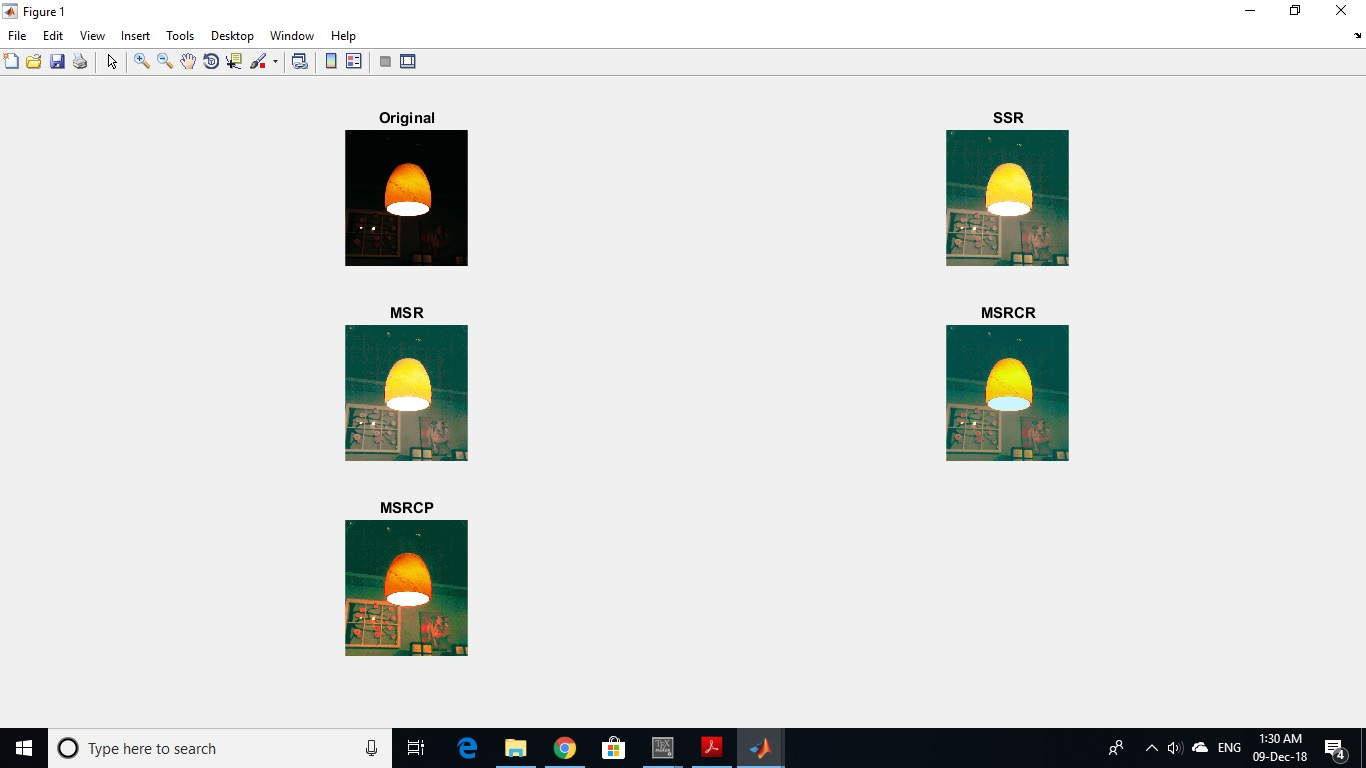
\includegraphics[scale=0.5]{images/ch3/retinexModel.jpg}
	\caption{Result of Retinex Model}
\end{figure}

\section{Power Law Transformation}
Image enhancement can be carried out in the spatial or the Fourier domains and one of the important
parameters to be looked at in this context is contrast enhancement\cite{pt1}. In the spatial domain,
the methods used may be further classified into: gray level transformations, histogram processing,
etc. As mentioned above, histogram equalization suffers from the fact that it may sometimes
decrease the contrast\cite{pt2}. Histogram specification or matching can be tailor-made to suit the images but requires lot of user input. Similarly, power law transformations or piece-wise linear transformation
functions also require lot of user input\cite{pt3}. In the former case one has to choose the exponent
appearing in the transformation function, while in the latter case one has to choose the slopes
and ranges of the straight lines which form the transformation function\cite{pt2}.

The power-law transformation is usually defined as

\begin{equation}
	s=c \thinspace r^\gamma
\end{equation}
where $s$ and $r$ are the gray levels of the pixels in the output and the input images, respectively and
$c$ is a constant. These power law transformation functions are shown graphically in the diagram
(figure \ref{fig:powerLawTransformation}).
Figure \ref{fig:powerLawTransformation} shows the plot of power law transformation with the input gray level $r$ along the $x$ axis and the output gray level $s$ on the $y$ axis for various values of $\gamma$ .
We will now consider that these transformations are applied on a low contrast image. We
assume that the background and foreground peaks have almost merged together in such a low
contrast image. Let $r_{max}$ be the dominant peak in the histogram\cite{he2}. If $r_{max}$ has a large value (in the
range $150\textrm{--}255$), then it is seen from the above graph that contrast stretching occurs by choosing
$\gamma \textgreater 1$ whereas for dark images ($r_{max}$ lies in the range $0\textrm{--}100$), we see that choosing $\gamma \textless 1$ leads
to contrast stretching. We can of course, automate this procedure for choosing the appropriate
exponent, by finding out the peak value in the histogram. However, we can further generalize
this procedure so that the most appropriate value of the exponent is chosen\cite{pt3}.

\begin{figure}
	\centering
	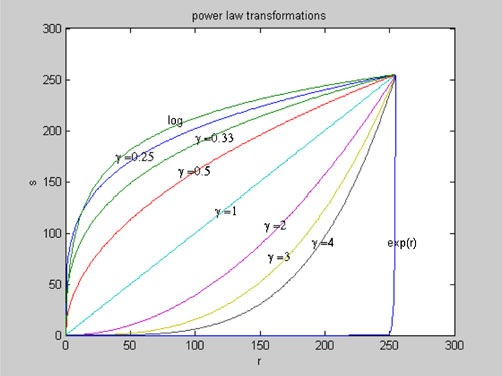
\includegraphics[scale=0.9]{images/ch3/powerLawTransformation.jpg}
	\caption{Plot of power law transformation for various $\gamma$ with input gray level along $X$ axis and output
gray level along $Y$ axis.}
	\label{fig:powerLawTransformation}
\end{figure}

\section{Histogram Equalization}
An image histogram is a type of histogram that acts as a graphical representation of
the tonal distribution in a digital image\cite{he1}. It plots the number of pixels for each tonal
value. A histogram is a representation of a frequency distribution\cite{he2}. The histogram
of a digital image with $G$ total possible intensity levels in the $[0,G − 1]$ is defined
as the discrete function:

\begin{equation}
	p(\gamma_{k})=\frac{n_{k}}{n}
\end{equation}

Where $\gamma_{k}$ is the intensity level in the original raw image $n_{k}$ is the number of
pixels in the image whose intensity level is n is the total no of pixels\cite{he2}.

Histogram equalization is used to enhance the contrast of the image, it spreads the
intensity values over full range. Histogram equalization technique can’t be used for
images suffering from non-uniform illumination in their backgrounds as this process
only adds extra pixels to the light regions of the image and removes extra pixels from
dark regions of the image resulting in a high dynamic range in the output image\cite{he1}.The
goal of histogram equalization is to spread out the contrast of a given image evenly
throughout the entire available dynamic range\cite{he2}.

\begin{figure}
	\centering
	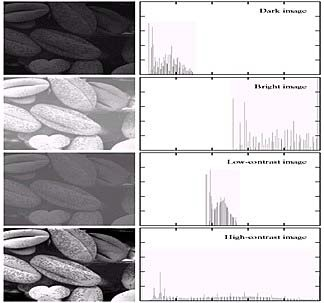
\includegraphics[scale=1]{images/ch3/histogramEqualization.jpg}
	\caption{Seed Image and its histogram}
	\label{fig:histogramEqualization}
\end{figure}

In histogram equalization technique, it is the probability density function (pdf)
that is being manipulated. To make it simple, what histogram equalization technique
does is that, it changes the pdf of a given image into that of a uniform probability
density function that spreads out from the lowest pixel value ($0$ in this case) to
the highest pixel value $(L − 1)$ . This can be achieved quite easily if the pdf is a
continuous function\cite{he1}. However, since we are dealing with a digital image, the pdf
will be a discrete function. Lets suppose we have an image $x$ , and let the dynamic
range for the intensity $\gamma_{k}$ varies from $0$ (black) to $L1$ (white). This pdf can be
approximated using the probability based on the histogram $p(\gamma_{k})$ as follow:

\begin{equation}
	pdf(x)=p(\gamma_{k})= \frac{total\;pixels\;with\;intensity\; \gamma_{k}}{total\;pixels\;I\;image\;x}
\end{equation}

From this pdf, we can then obtain the cumulative density function (cdf) as follows:

\begin{equation}
	cdf(x)=\sum_{k=0}^{L-1}p(\gamma_{k})
\end{equation}

Where $p(\gamma_{k})$ is the probability for pixel of intensity. The output of a pixel from
the histogram equalization operation is then equal to the cdf of the image or mathematically\cite{he2} :

\begin{equation}
	p(s_{k})=\sum_{k=0}^{L-1}p(\gamma_{k})
\end{equation}

To get the value of the pixel, $p(s_{k})$ needs to be multiplied by $L1$ and then round
it to the nearest integer

\subsection{Equalization on Color Image}
\begin{itemize}
	\item \textbf{Equalize R, G, B components independently (method1)}\\
			This scheme is one of the mostly used methods for color image processing.
			Each channels of RGB space are processed using Histogram Equalization
			independently[2].After the Equalize the R,G,B components we concate all the three
			components and get the better image compare to input image.

			\begin{figure}
				\centering
				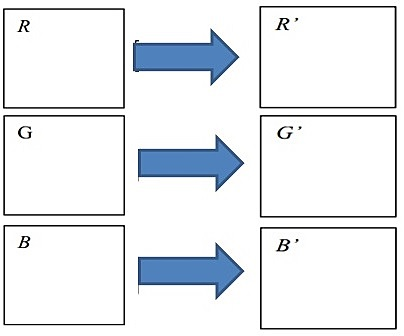
\includegraphics[scale=1]{images/ch3/method1.jpg}
				\caption{Block diagram showing the implementation of Method 1}
				\label{method1}
			\end{figure}
	\item \textbf{Equalize tha V Component from HSV Color Space (method 2)}\\
			In order to process color image in RGB color space using this scheme, image first
			must be transformed to hue, saturation and luminance (HSV) color space.Here	
			Brightness is a synonym of intensity. Hue represents the impression related to the
			dominant wavelength of the color stimulus Saturation shows the relative color purity
			(amount of white light in the color).
			Hue and Saturation taken together are called the chromaticity coordinates (polar
			system).
			In this method we apply the Histogram Equalization on V component on HSV
			color space .After the Equalize the V we combine the V with H and S .Then we get
			the better image compare to input image.\\
			$HSV \rightarrow H, S, V$\\
			$V \rightarrow V(equalize)$\\
			$HSV(equalize) \rightarrow H, S, V(equalize)$\\
	\item \textbf{Equalize the Y Component from YIQ Color Space(method 3)}\\
			In order to process color image in RGB color space using this scheme, the image
			first must be transformed to YIQ color space[4][5].\\
			Here\\
			The Y component represents the luma information, and is the only component used
			by black-and-white television receivers.\\
			I stands for in-phase\\
			Q stands for quadrature\\
			I and Q represent the chrominance information.\\

			In this method we apply the Histogram Equalization on Y component on YIQ
			color space .After the Equalize the Y we combine the Y with I and Q .Then we get the better image compare to 				input image.\\
			$YIQ \rightarrow YIQ$\\
			$Y \rightarrow Y(equalize)$\\
			$YIQ(equalixe) \rightarrow Y, I, Q(equalize)$\\
\end{itemize}

\section{Adaptive Histogram Equalization(AHE) method}
This is an extension to traditional Histogram Equalization
technique. It enhances the contrast of images by transforming
the values in the intensity image I \cite{ie1}. Unlike HISTEQ, it operates
on small data regions (tiles), rather than the entire image. Each
tile's contrast is enhanced, so that the histogram\cite{he1} of the output
region approximately matches the specified histogram. The
neighboring tiles are then combined using bilinear interpolation
in order to eliminate artificially induced boundaries.
The contrast, especially in homogeneous areas, can be limited
in order to avoid amplifying the noise which might be present
in the image\cite{he2}.
\begin{itemize}
	\item Algorithm Steps:
	\begin{enumerate}
		\item Obtain all the inputs: Image, Number of regions in row and column directions, Number of bins for the 	
		histograms used in building image transform function (dynamic range), Clip limit for contrast limiting (normalized 	
		from 0 to 1)
		\item Pre-process the inputs: Determine real clip limit from the normalized value if necessary, pad the image 
		before splitting it into regions
		\item Process each contextual region (tile) thus producing gray level mappings: Extract a single image region, make 
		a histogram for this region using the specified number of bins, clip the histogram using clip limit, create a 
		mapping (transformation function) for this region.
		\item Interpolate gray level mappings in order to assemble final CLAHE image: Extract cluster of four neighbouring 
		mapping functions, process image region partly overlapping each of the mapping tiles, extract a single pixel, apply
		four mappings to that pixel, and interpolate between the results to obtain the output pixel; repeat over the entire 
		image.
	\end{enumerate}
\end{itemize}

In low contrast images, the features of interest may occupy only a
relatively narrow range of gray scale, with the majority of gray levels occupied by
“uninteresting areas” such as background and noise. These “uninteresting areas”
may also generate large counts of pixels and hence, large peaks in the
histogram\cite{he2}. In this case, the global histogram equalization amplifies the image
noise and increases visual graininess or patchiness. The global histogram
equalization technique does not adapt to local contrast requirements, and minor
contrast differences can be entirely missed when the number of pixels falling in a
particular gray range is small\cite{he2}.

Adaptive Histogram Equalization (AHE) is a modified histogram
equalization procedure that optimizes contrast enhancement based on local
image data. The basic idea behind the scheme is to divide the image into a grid
of rectangular contextual regions, and to apply a standard histogram equalization
in each. The optimal number of contextual regions and the size of the regions
depend on the type of input image, and the most commonly used region size is
8x8 (pixels)\cite{he2}. In addition, a bi-linear interpolation scheme is used to avoid
discontinuity issues at the region boundaries\cite{he2}.

Figure \ref{fig:bilinearInterpolation} illustrates the application of the interpolation scheme at the
boundaries. Gray level assignment at the sample positions indicated by the white
dot are derived from gray-value distributions in the surrounding contextual regions\cite{he2}. The points A, B, C, and D are the centers of the surrounding contextual
regions; region-specific gray level mappings (gA(s), gB(s), gC(s) and gD(s)) are
based on the histogram equalization of the pixels contained. Thus, assuming that
the original pixel intensity at the sample point is s, its new gray value s’ is
calculated by bilinear interpolation of the gray-level mappings that were
calculated for each of the surrounding contextual regions:

\begin{equation}
	s'=(1-y)((1-x)g_{A}(s) + xg_{B}(s))+y(((1-x)g_{c}(s)+xg_{D}(s))
\end{equation}

where x and y are normalized distances with respect to the point A. This
gray level interpolation is repeated over the entire image

\begin{figure}
	\centering
	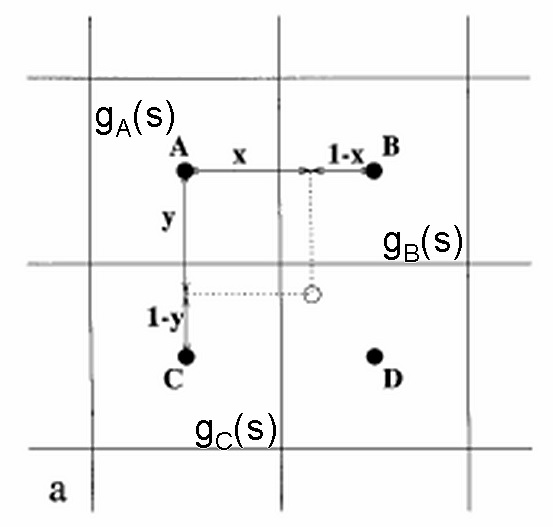
\includegraphics[scale=0.7]{images/ch3/bilinearInterpolation.jpg}
	\caption{Bilinear interpolation to eliminate region boundaries[From Zuiderveld, 1994].}
	\label{fig:bilinearInterpolation}
\end{figure}

AHE is able to overcome the limitations of the standard equalization
method as discussed earlier, and achieves a better presentation of information
present in the image. However, AHE is unable to distinguish between noise and
features in the local contextual regions. Hence, background noise is amplified in
“flat” or “featureless” regions of the image, which is a major drawback of the
method\cite{he2}.

\subsection{Contrast Limited Adaptive Histogram Equalization (CLAHE)}
The noise problem associated with AHE can be reduced by limiting
contrast enhancement specifically in homogeneous areas. These areas can be
characterized by a high peak in the histogram associated with the contextual
regions since many pixels fall inside the same gray level range. The Contrast
Limited Adaptive Histogram Equalization (CLAHE) limits the slope associated
with the gray level assignment scheme to prevent saturation, as illustrated in
Figure \ref{CLAHE}. This process is accomplished by allowing only a maximum number of
pixels in each of the bins associated with the local histograms. After “clipping” the
histogram, the clipped pixels are equally redistributed over the whole histogram
to keep the total histogram count identical\cite{he2}.
\begin{figure}
	\centering
	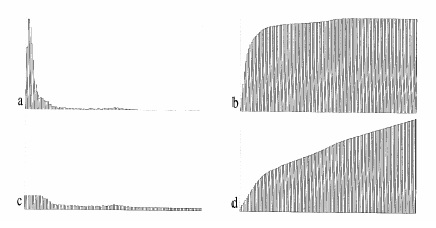
\includegraphics[scale=1]{images/ch3/CLAHE.jpg}
	\caption{Principle of contrast limiting as used in CLAHE. (a)
Histogram of a contextual region containing many background pixels.
(b) Calculated cumulative histogram. (c) Clipped histogram with excess
pixels redistributed throughout the histogram. (d) Cumulative clipped
histogram with maximum slope set to the clip limit [From Zuiderveld,
1994].}
\label{CLAHE}
\end{figure}

The clip limit is defined as a multiple of the average histogram contents
and is actually a contrast factor. Setting a very high clip limit basically limits the clipping and the process becomes a standard AHE technique\cite{he1}. A clip or contrast
factor of one prohibits any contrast enhancement, preserving the original image.
The main advantages of the CLAHE transform are its modest
computational requirements, ease of use and excellent results on most images. The CLAHE image has less amplified noise and avoids the brightness saturation in the standard histogram equalization\cite{he1}.

CLAHE does have its limitations. Since the method is aimed at optimizing
contrast, there no direct 1-to-1 relationship between the gray values of the
original image and the CLAHE processed result\cite{he2}. Pixels of the same gray level in
the original image may be mapped to different gray levels in the output image,
because of the equalization process and bilinear interpolation. Consequently,
CLAHE images are not suited for quantitative measurements that rely on
physical meaning of image intensity.


\chapter{Implementation}
Retinex Theory was formulated by Edwin H. Land In 1964. His theory and an extension, the “reset Retinex” were further formalized by Land and Mc Cann [1]. It was the first attempt to simulate and explain the human visual system how it perceives colours, based on experiments using Mondrian patterns [3].
\section{Introduction}
Besides digital photography, retinex algorithms are used to make the information in astronomical photos visible and detect, in medicine, poorly visible structures in X-rays or scanners. In brief it helps to achieve many features such as sharpening, colour constancy processing and dynamic range compression [5]. The Retinex Image Enhancement Algorithm is an automatic image enhancement method that enhances a digital image in terms of dynamic range compression, colour independence from the spectral distribution of the scene illuminate, and colour/ lightness rendition. The digital image enhanced by the Retinex Image Enhancement Algorithm is much closer to the scene perceived by the human visual system, under all kinds and levels of lighting variations, than the digital image enhanced by any other method [6]. Image enhancement technology has permeated in many areas of science, engineering and civilian, such as biomedicine images, astrophotography, satellite pictures, computer vision, surveillance systems, civilian cameras, etc.[7]

\section{Problem Definition}
Our system will enhance the input image by applying retinex algorithms: Multi-Scale Retinex with color Restoration (MSRCR), Multi-scale Retinex with Chromaticity Preservation (MSRCP) and Automated Multi-Scale Retinex with Color Restoration (AMSRCR). Thus, the Problem definition can be proposed as follows: To implement the Algorithms: MSRCR, MSRCP and AMSRCR. Also, these algorithms require implementation of Single-Scale Retinex (SSR) algorithm and the SimplestColorBalance algorithm [35].
\section{Objective}
	\begin{itemize}
		\item To implement Single-Scale Retinex and Color Restoration Algorithms.
		\item To implement Multi-Scale Retinex with Color Restoration using above 
		algorithms (MSRCR).
		\item To implement Multi-Scale retinex with Chromaticity preservation- MSRCP.(a 
		modified version of above algorithm).
		\item To implement Automated Multi-Scale Retinex with Color Restoration algorithm.	
		(An automated (image independent) approach to MSRCR)- AMSRCR.
	\end{itemize}
	
\section{Scope}
The Retinex Image Enhancement Algorithm is an automatic image enhancement method that enhances a digital image in terms of dynamic range compression, colour independence from the spectral distribution of the scene illuminate, and colour/ lightness rendition. So, the scope of this project is to implement the Retinex based image Enhancement Algorithms, which involves the implementation of following three models of retinex algorithms:
	\begin{itemize}
		\item Multi-Scale Retinex algorithm with color Restoration (MSRCR)
		\item Multi-Scale Retinex algorithm with Chromaticity Preservation (MSRCP)
		\item Automated Multi-Scale Retinex algorithm with Color Restoration (AMSRCR)

	\end{itemize}
\section{Existing System}
The existing image enhancement techniques like auto gain/offset, gamma correction, histogram equalization and homomorphic filtering heavily depend on input images. For auto gain/offset, it could achieve dynamic range compression but at the loss of details due to saturation and clipping. For gamma correction, it is good to improve pictures either too dark or too bright but it is a global function applied to the picture, thus there is no enhancement involved. For histogram equalization and homomorphic filtering, they all failed for bi-modal pictures, which include both dark and bright areas. But for retinex, it could achieve satisfactory results for both pictures, thus its benefits are obviously to see.[8]
\section{Outline}
This project report is organized into six chapters: Chapter 1 introduces the project; chapter 2 describes related work and reviews previous works; Chapter 3 presents the technology that will be used. Chapter 4 presents the system analysis and design in detail, chapter 5 presents the results and Chapter 6 is the Conclusion.
\chapter{Result and Discussion}
Retinex Theory was formulated by Edwin H. Land In 1964. His theory and an extension, the “reset Retinex” were further formalized by Land and Mc Cann [1]. It was the first attempt to simulate and explain the human visual system how it perceives colours, based on experiments using Mondrian patterns [3].
\section{Introduction}
Besides digital photography, retinex algorithms are used to make the information in astronomical photos visible and detect, in medicine, poorly visible structures in X-rays or scanners. In brief it helps to achieve many features such as sharpening, colour constancy processing and dynamic range compression [5]. The Retinex Image Enhancement Algorithm is an automatic image enhancement method that enhances a digital image in terms of dynamic range compression, colour independence from the spectral distribution of the scene illuminate, and colour/ lightness rendition. The digital image enhanced by the Retinex Image Enhancement Algorithm is much closer to the scene perceived by the human visual system, under all kinds and levels of lighting variations, than the digital image enhanced by any other method [6]. Image enhancement technology has permeated in many areas of science, engineering and civilian, such as biomedicine images, astrophotography, satellite pictures, computer vision, surveillance systems, civilian cameras, etc.[7]

\section{Problem Definition}
Our system will enhance the input image by applying retinex algorithms: Multi-Scale Retinex with color Restoration (MSRCR), Multi-scale Retinex with Chromaticity Preservation (MSRCP) and Automated Multi-Scale Retinex with Color Restoration (AMSRCR). Thus, the Problem definition can be proposed as follows: To implement the Algorithms: MSRCR, MSRCP and AMSRCR. Also, these algorithms require implementation of Single-Scale Retinex (SSR) algorithm and the SimplestColorBalance algorithm [35].
\section{Objective}
	\begin{itemize}
		\item To implement Single-Scale Retinex and Color Restoration Algorithms.
		\item To implement Multi-Scale Retinex with Color Restoration using above 
		algorithms (MSRCR).
		\item To implement Multi-Scale retinex with Chromaticity preservation- MSRCP.(a 
		modified version of above algorithm).
		\item To implement Automated Multi-Scale Retinex with Color Restoration algorithm.	
		(An automated (image independent) approach to MSRCR)- AMSRCR.
	\end{itemize}
	
\section{Scope}
The Retinex Image Enhancement Algorithm is an automatic image enhancement method that enhances a digital image in terms of dynamic range compression, colour independence from the spectral distribution of the scene illuminate, and colour/ lightness rendition. So, the scope of this project is to implement the Retinex based image Enhancement Algorithms, which involves the implementation of following three models of retinex algorithms:
	\begin{itemize}
		\item Multi-Scale Retinex algorithm with color Restoration (MSRCR)
		\item Multi-Scale Retinex algorithm with Chromaticity Preservation (MSRCP)
		\item Automated Multi-Scale Retinex algorithm with Color Restoration (AMSRCR)

	\end{itemize}
\section{Existing System}
The existing image enhancement techniques like auto gain/offset, gamma correction, histogram equalization and homomorphic filtering heavily depend on input images. For auto gain/offset, it could achieve dynamic range compression but at the loss of details due to saturation and clipping. For gamma correction, it is good to improve pictures either too dark or too bright but it is a global function applied to the picture, thus there is no enhancement involved. For histogram equalization and homomorphic filtering, they all failed for bi-modal pictures, which include both dark and bright areas. But for retinex, it could achieve satisfactory results for both pictures, thus its benefits are obviously to see.[8]
\section{Outline}
This project report is organized into six chapters: Chapter 1 introduces the project; chapter 2 describes related work and reviews previous works; Chapter 3 presents the technology that will be used. Chapter 4 presents the system analysis and design in detail, chapter 5 presents the results and Chapter 6 is the Conclusion.
\chapter{Conclusion}
In this thesis, methods that we applied balances the requirements of both appearance
enhancement and being faithful to the original appearance of an image has been
proposed and applied to the enhancement of full color images. Results have shown
the effectiveness of our algorithm in improving the contrast and colorfulness of
the original images. In this thesis, It is shown that we can get better image
from different Retinex Algorithms,Power Law Transformation, Histogram Equalization and Adaptive Histogram Equalization specification on color images gives us better results.

The Retinex Image Enhancement Algorithm is an automatic image enhancement method that enhances a digital image in terms of dynamic range compression, colour independence from the spectral distribution of the scene illuminate, and colour/ lightness rendition. The digital image enhanced by the Retinex Image Enhancement Algorithm is much closer to the scene perceived by the human visual system, under all kinds and levels of lighting variations, than the digital image enhanced by any other method.

%==================End Main Matters==================

%=================Back Matter========================
\bibliographystyle{plainnat}
%\bibliographystyle{plain}
%\bibliography{backMatter/myBib}

\begin{appendices}


\end{appendices}
\printnomenclature



\end{document}